\chapter{Visual design}\label{ch:visualDesign}
\section{Concept art}
Concept art was created for several iterations of the player-controlled pirate characters, some of which is seen in Figure \ref{fig:pirate_concepts}. They were drawn with a simple, cartoonish look in mind, so that the characters could easily catch the players' eyes. 

\begin{figure}[h!]
    \centering
    \begin{subfigure}[b]{0.2\textwidth}
		\centering        
        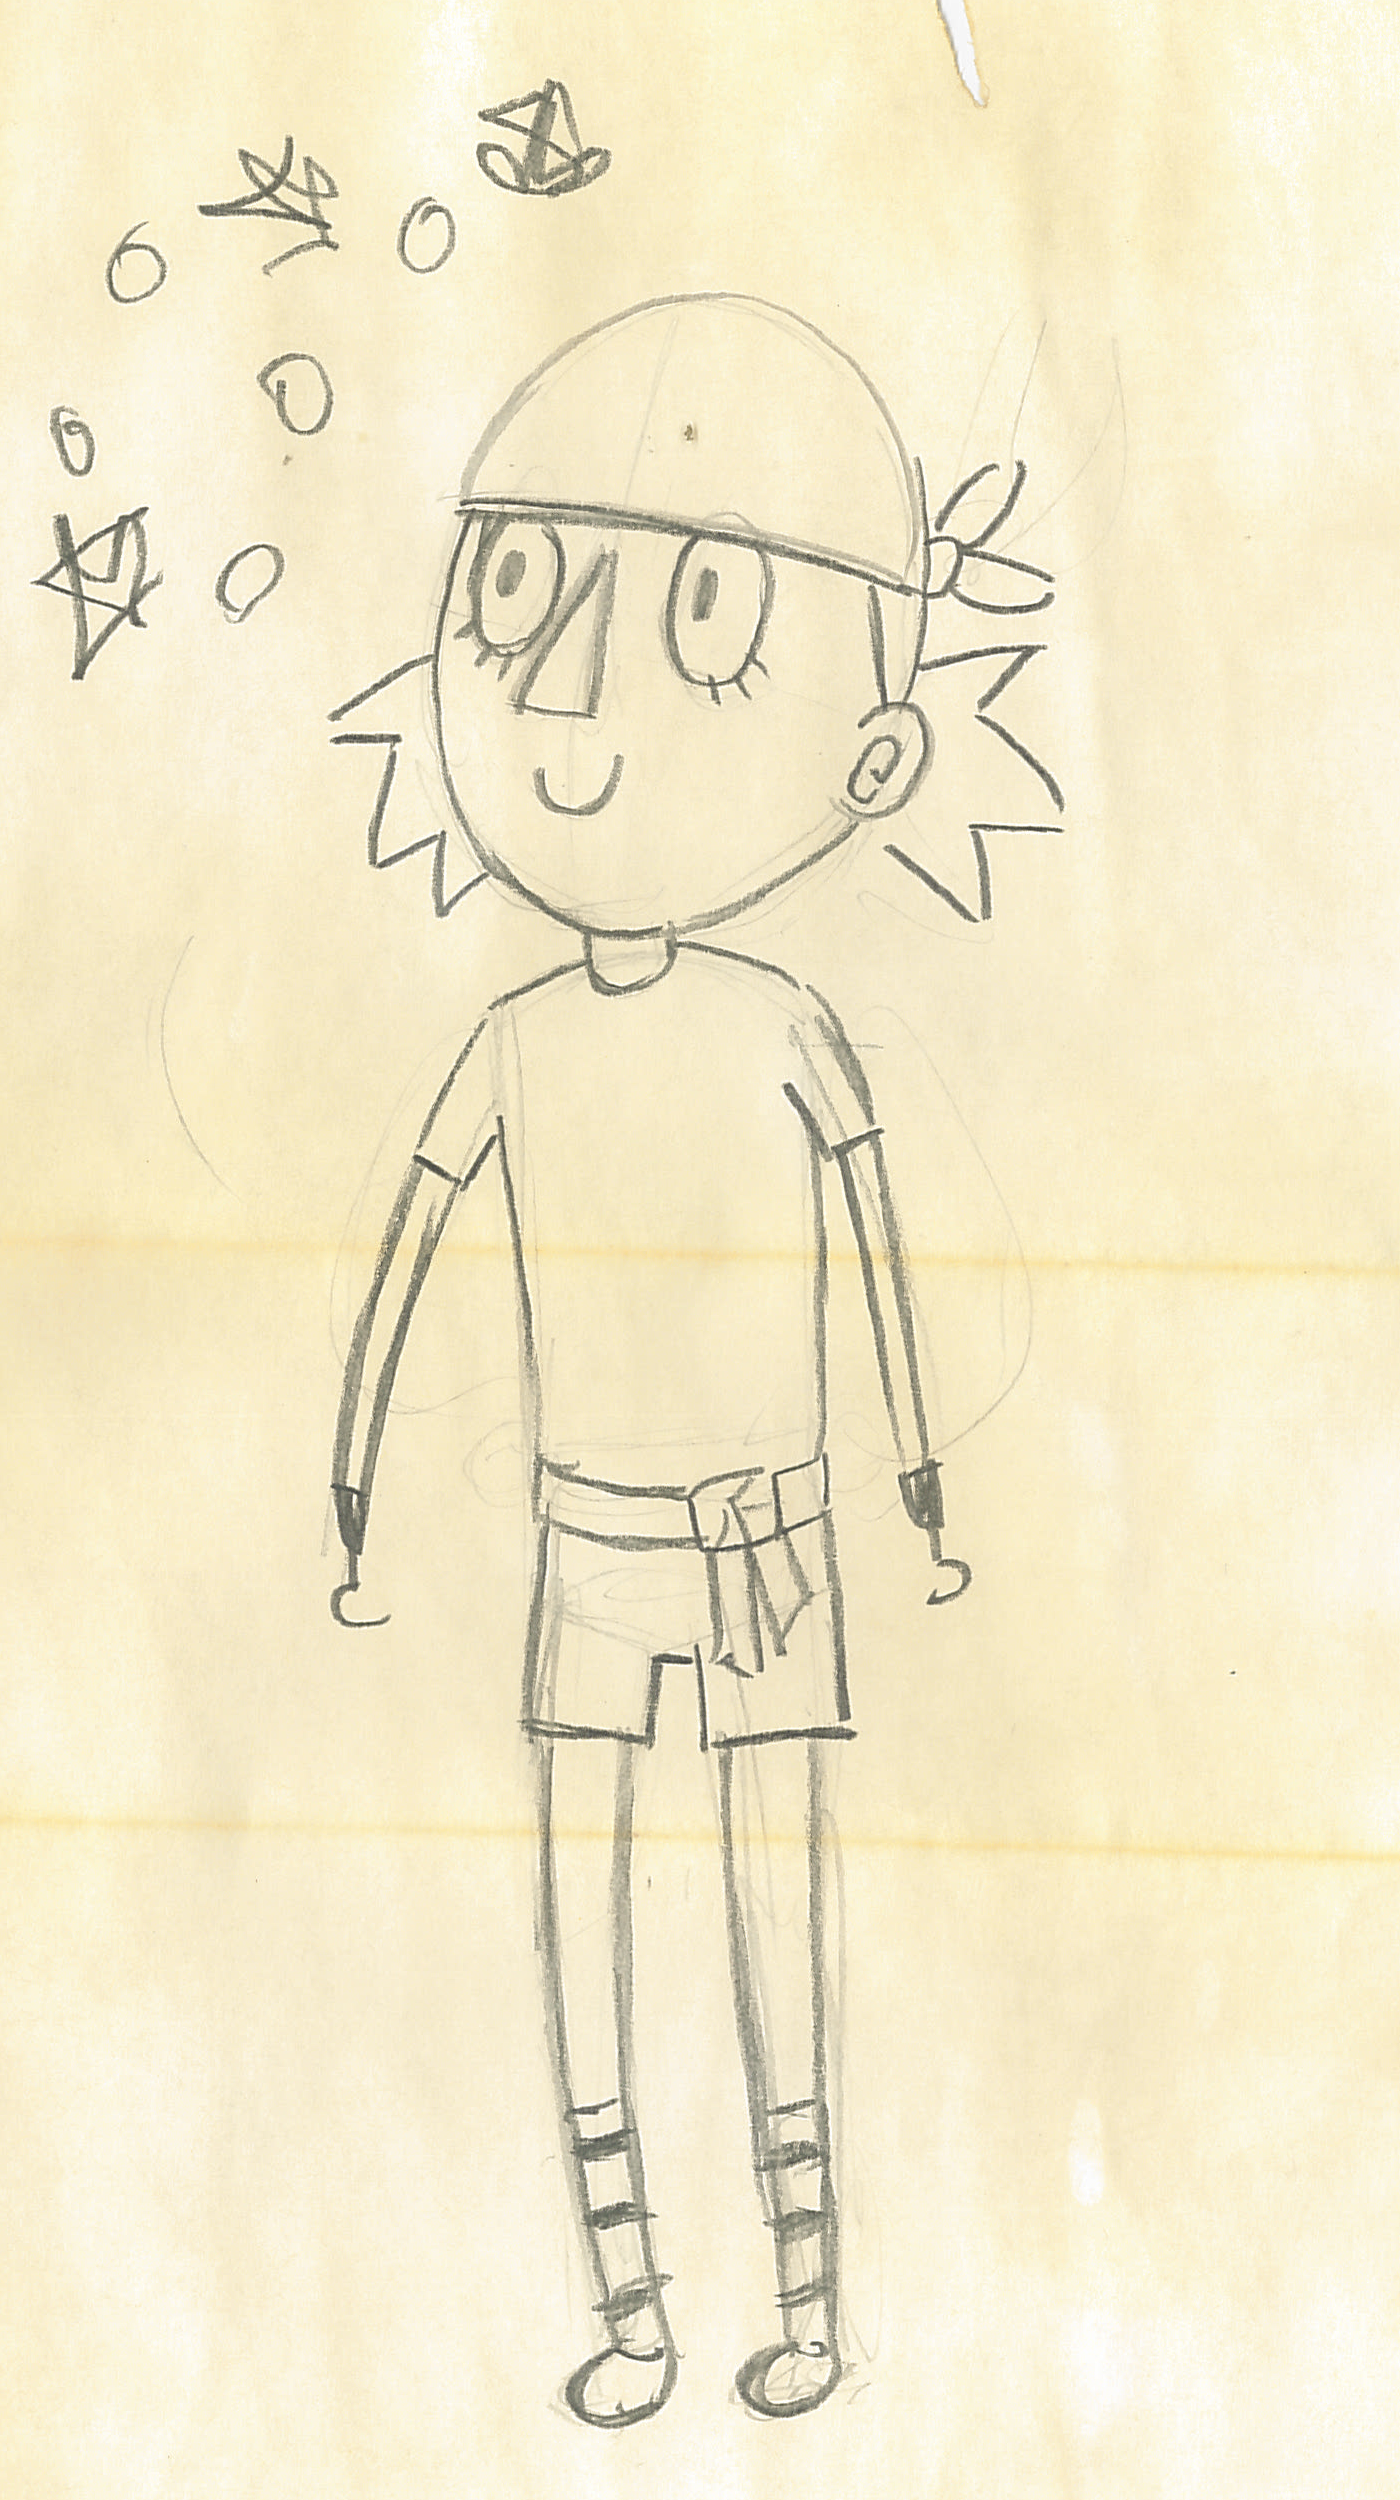
\includegraphics[width=\textwidth]{figures/pirate_concept_0.png}\caption{ \label{fig:pirate_concept_0}}
    \end{subfigure}
    \begin{subfigure}[b]{0.2\textwidth}
    	\centering
        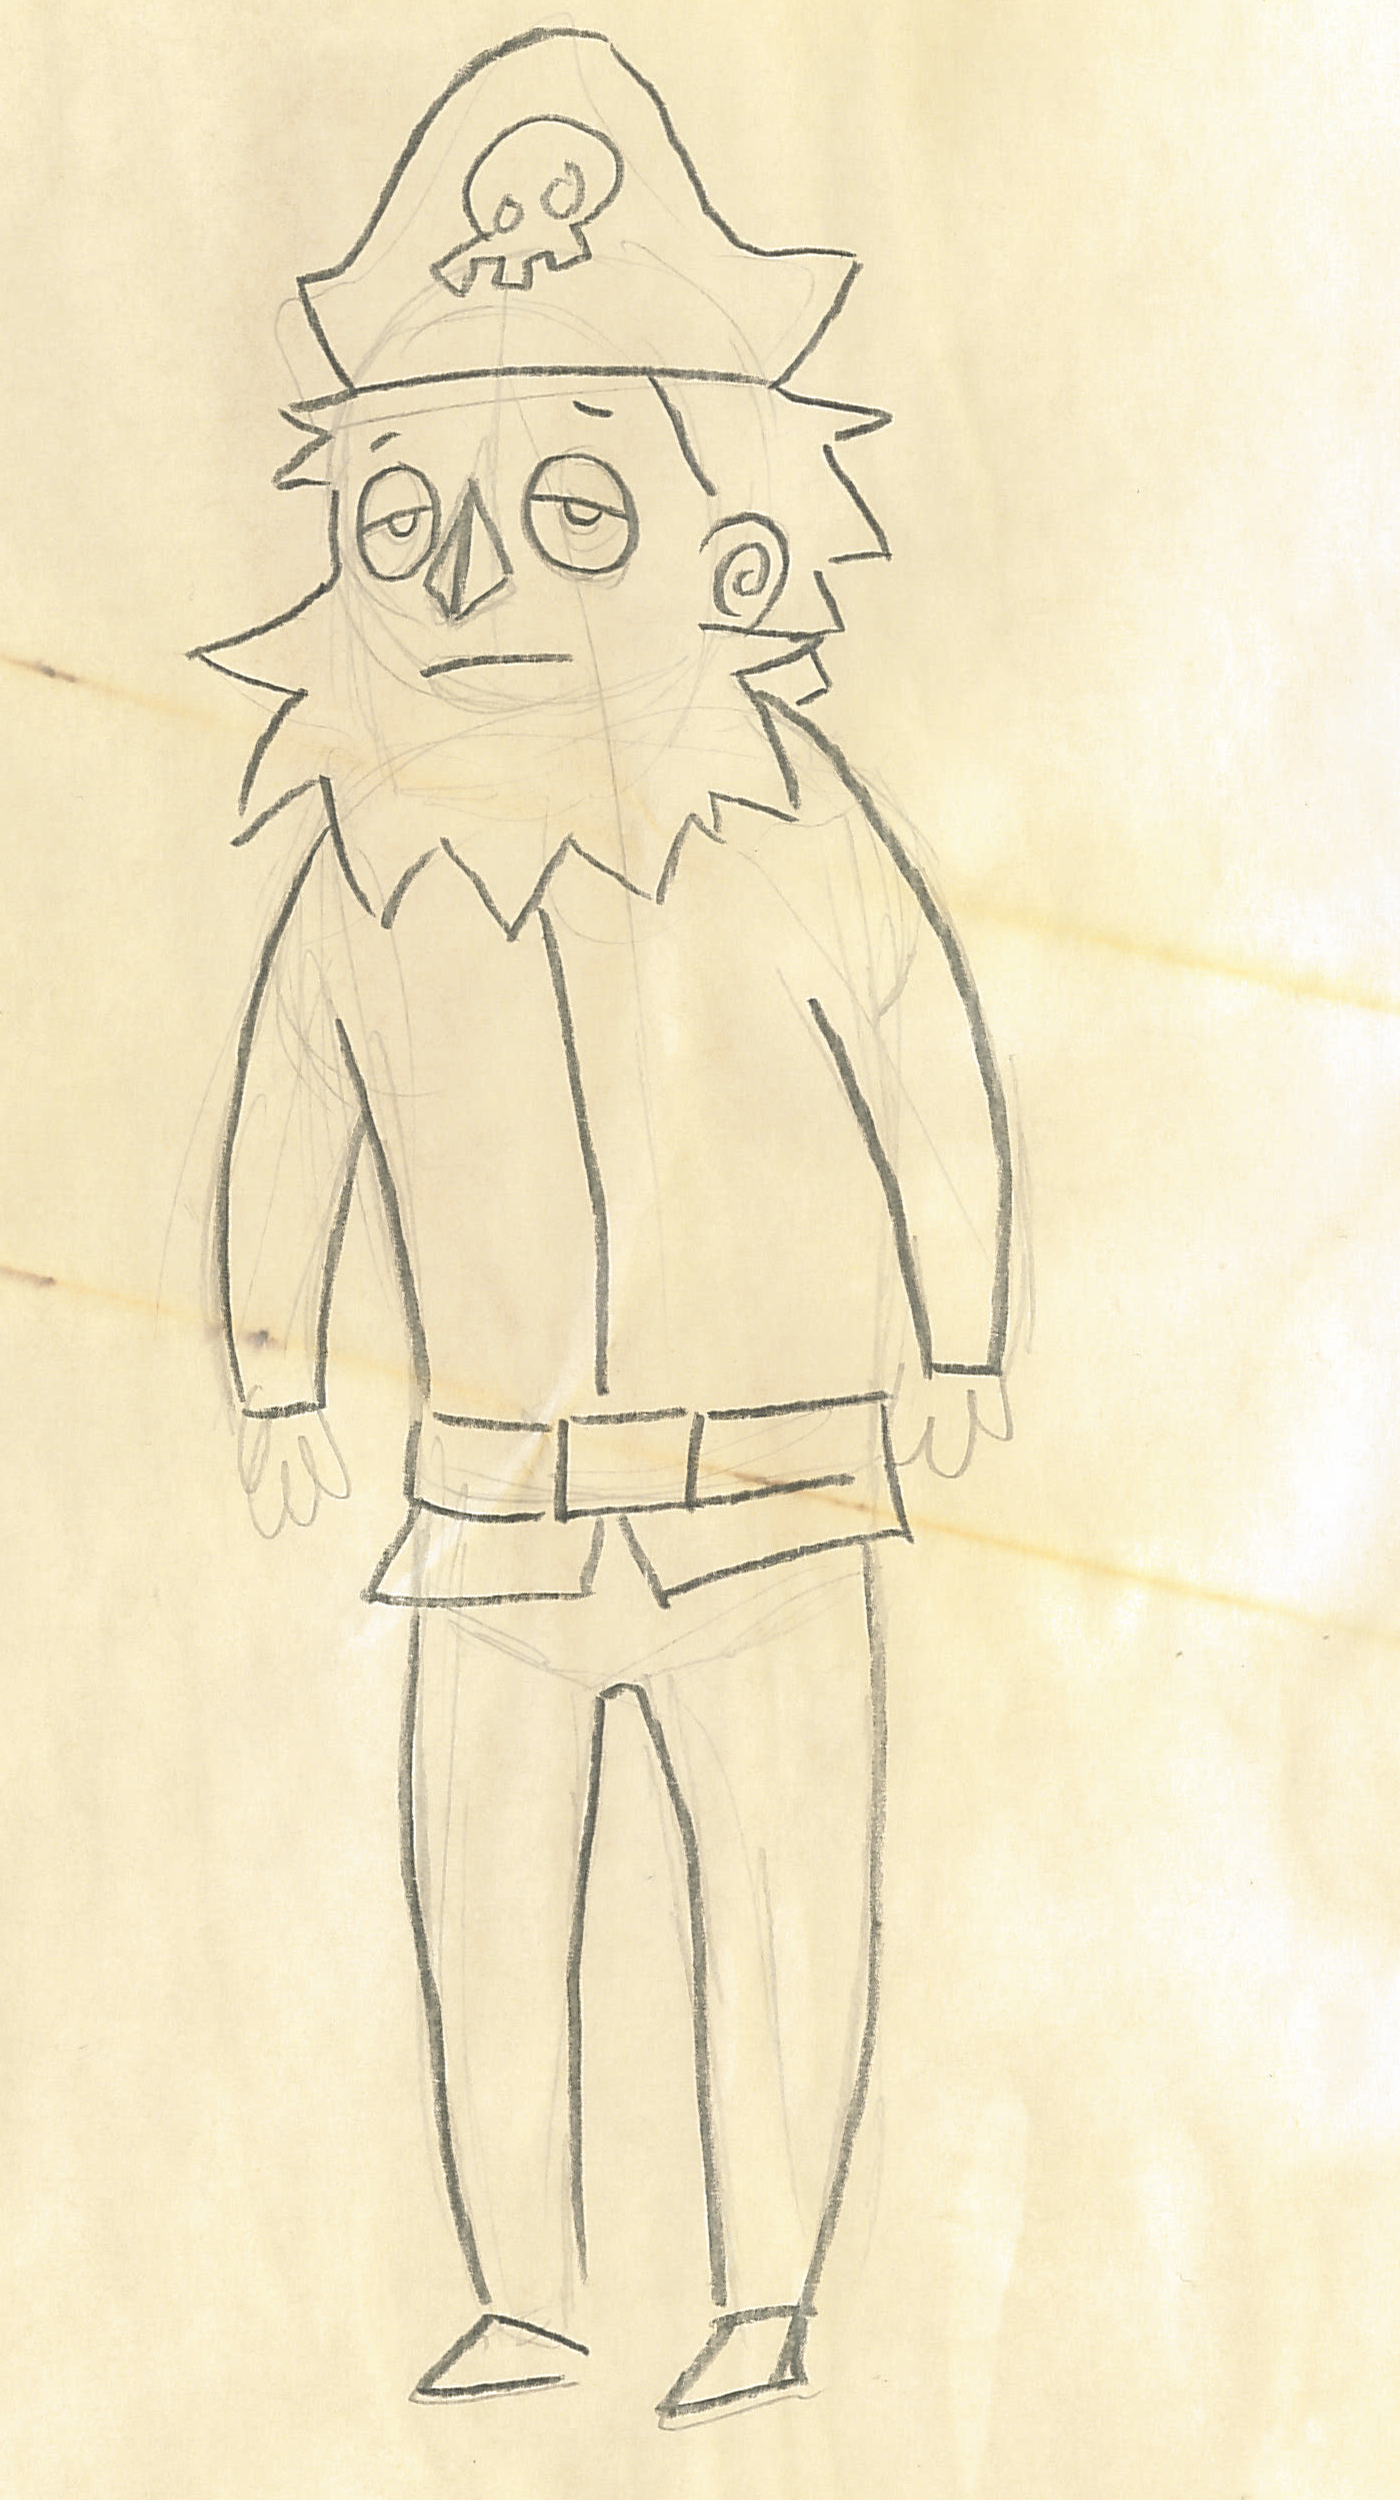
\includegraphics[width=\textwidth]{figures/pirate_concept_1.png}\caption{ \label{fig:pirate_concept_1}}
    \end{subfigure}
    \begin{subfigure}[b]{0.2\textwidth}
    	\centering
        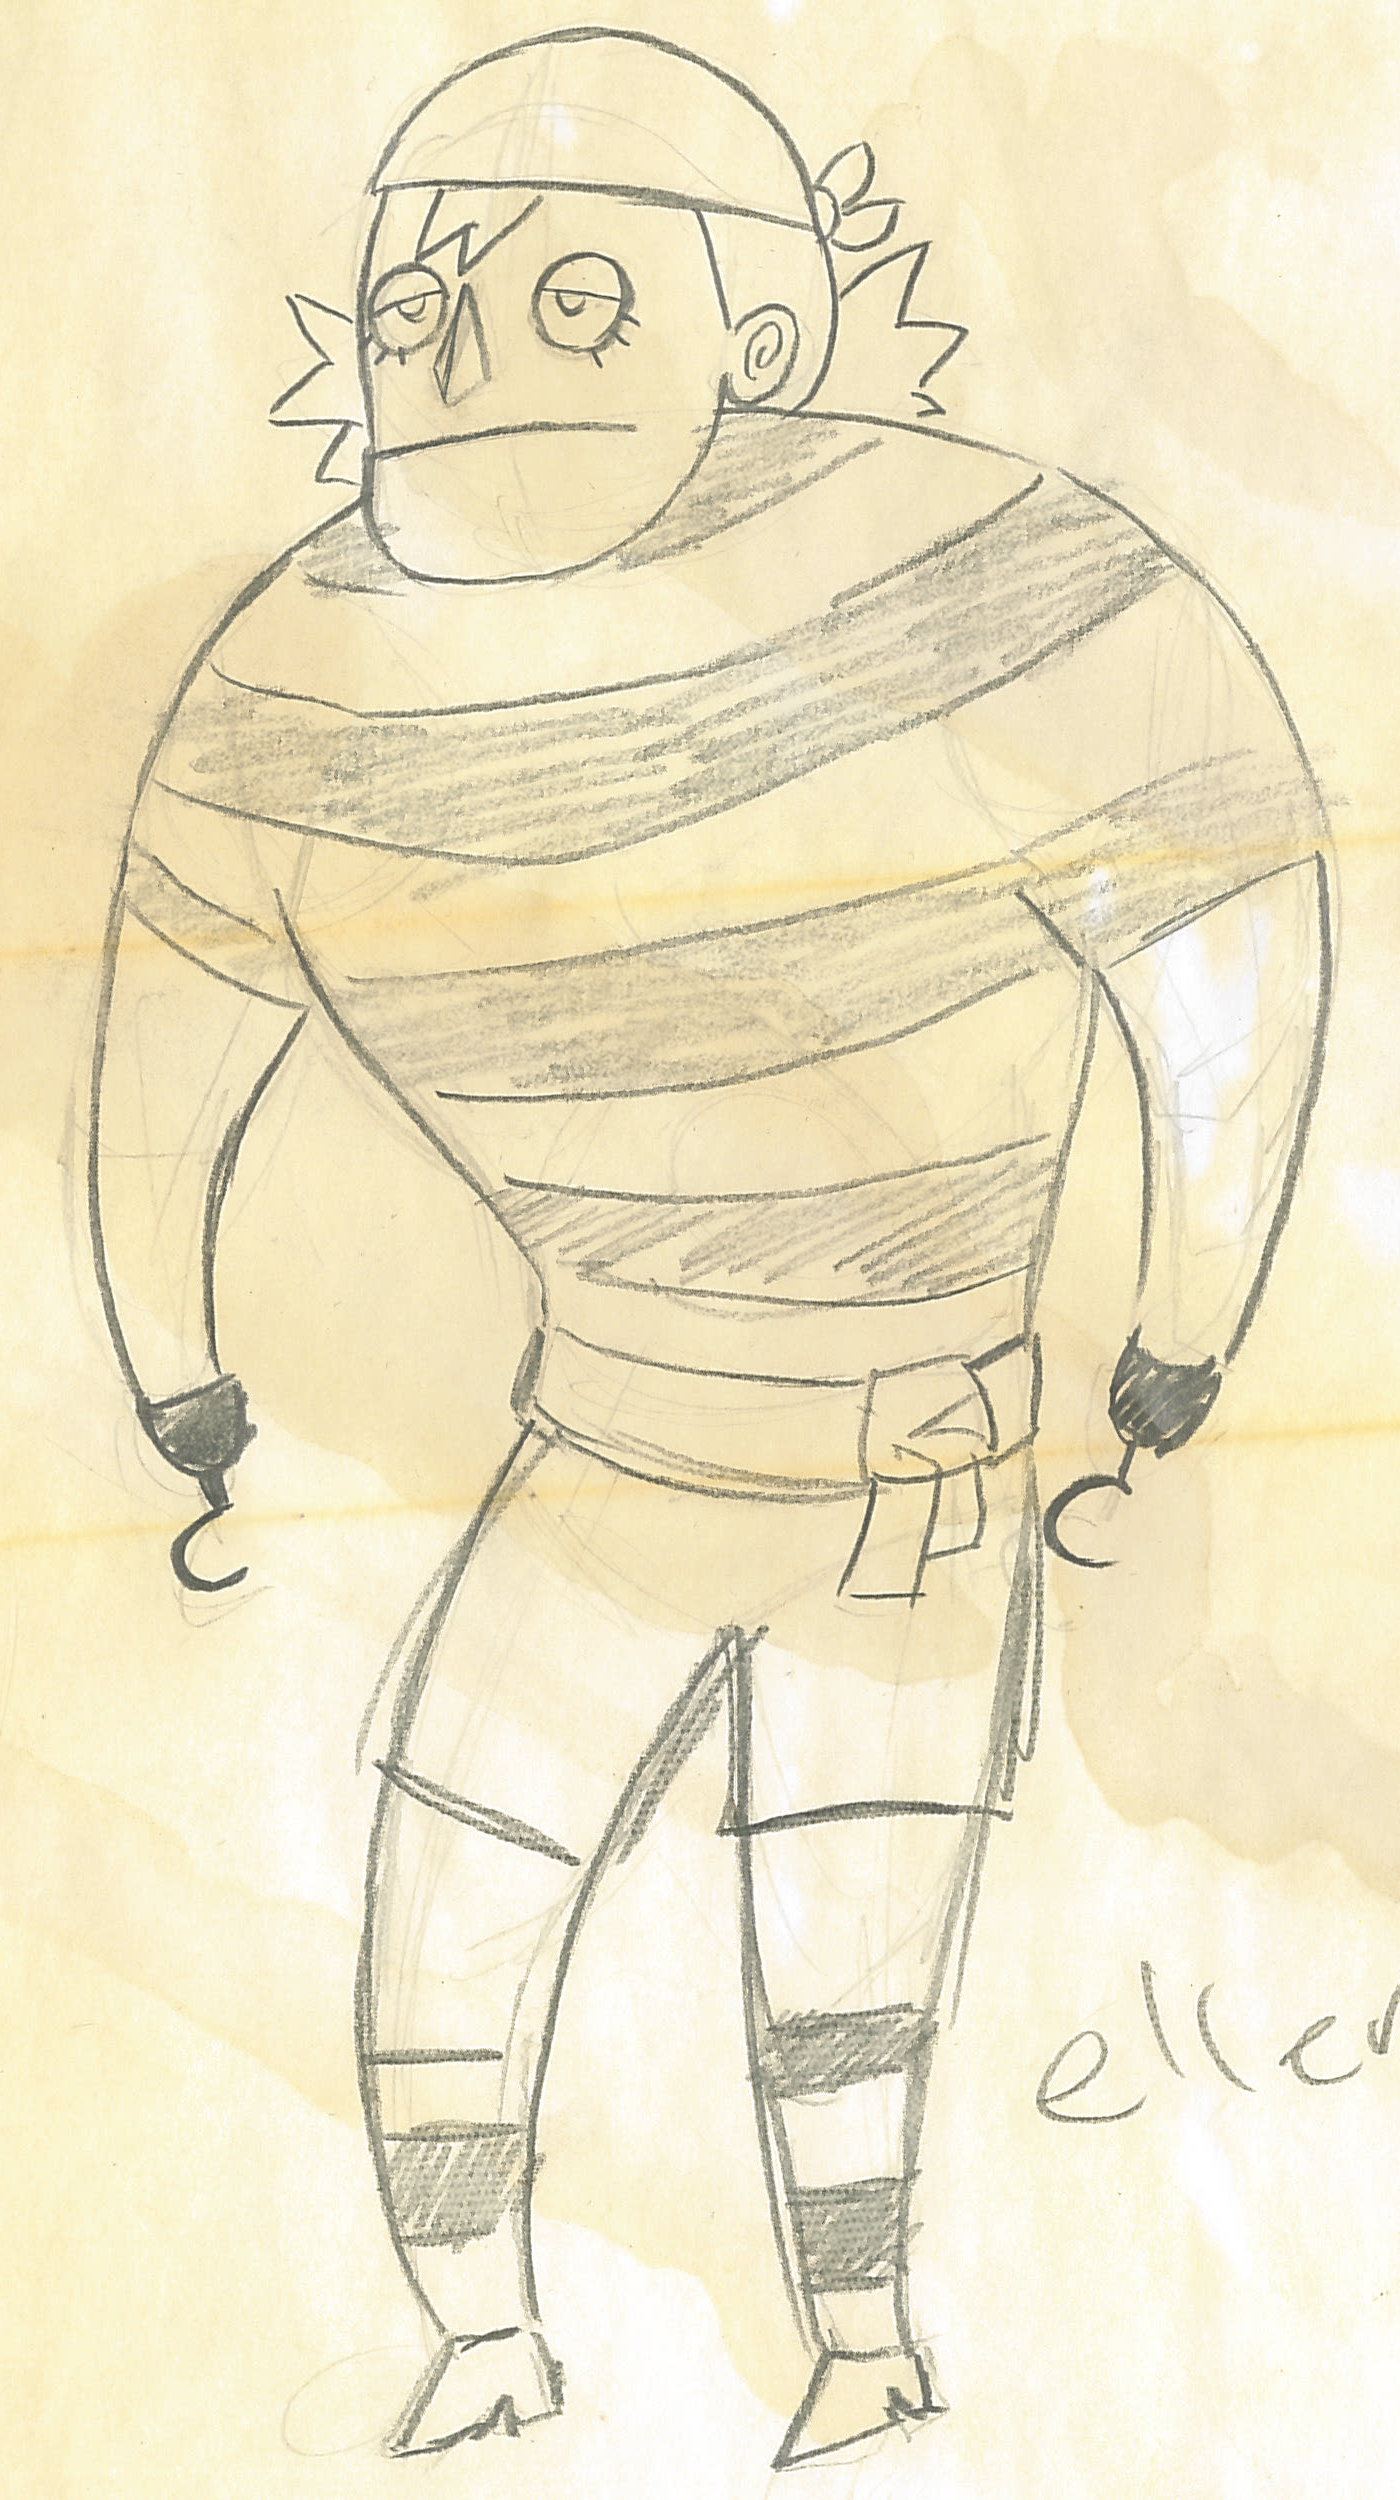
\includegraphics[width=\textwidth]{figures/pirate_concept_2.png}\caption{ \label{fig:pirate_concept_2}}
    \end{subfigure}
    \begin{subfigure}[b]{0.2\textwidth}
    	\centering
        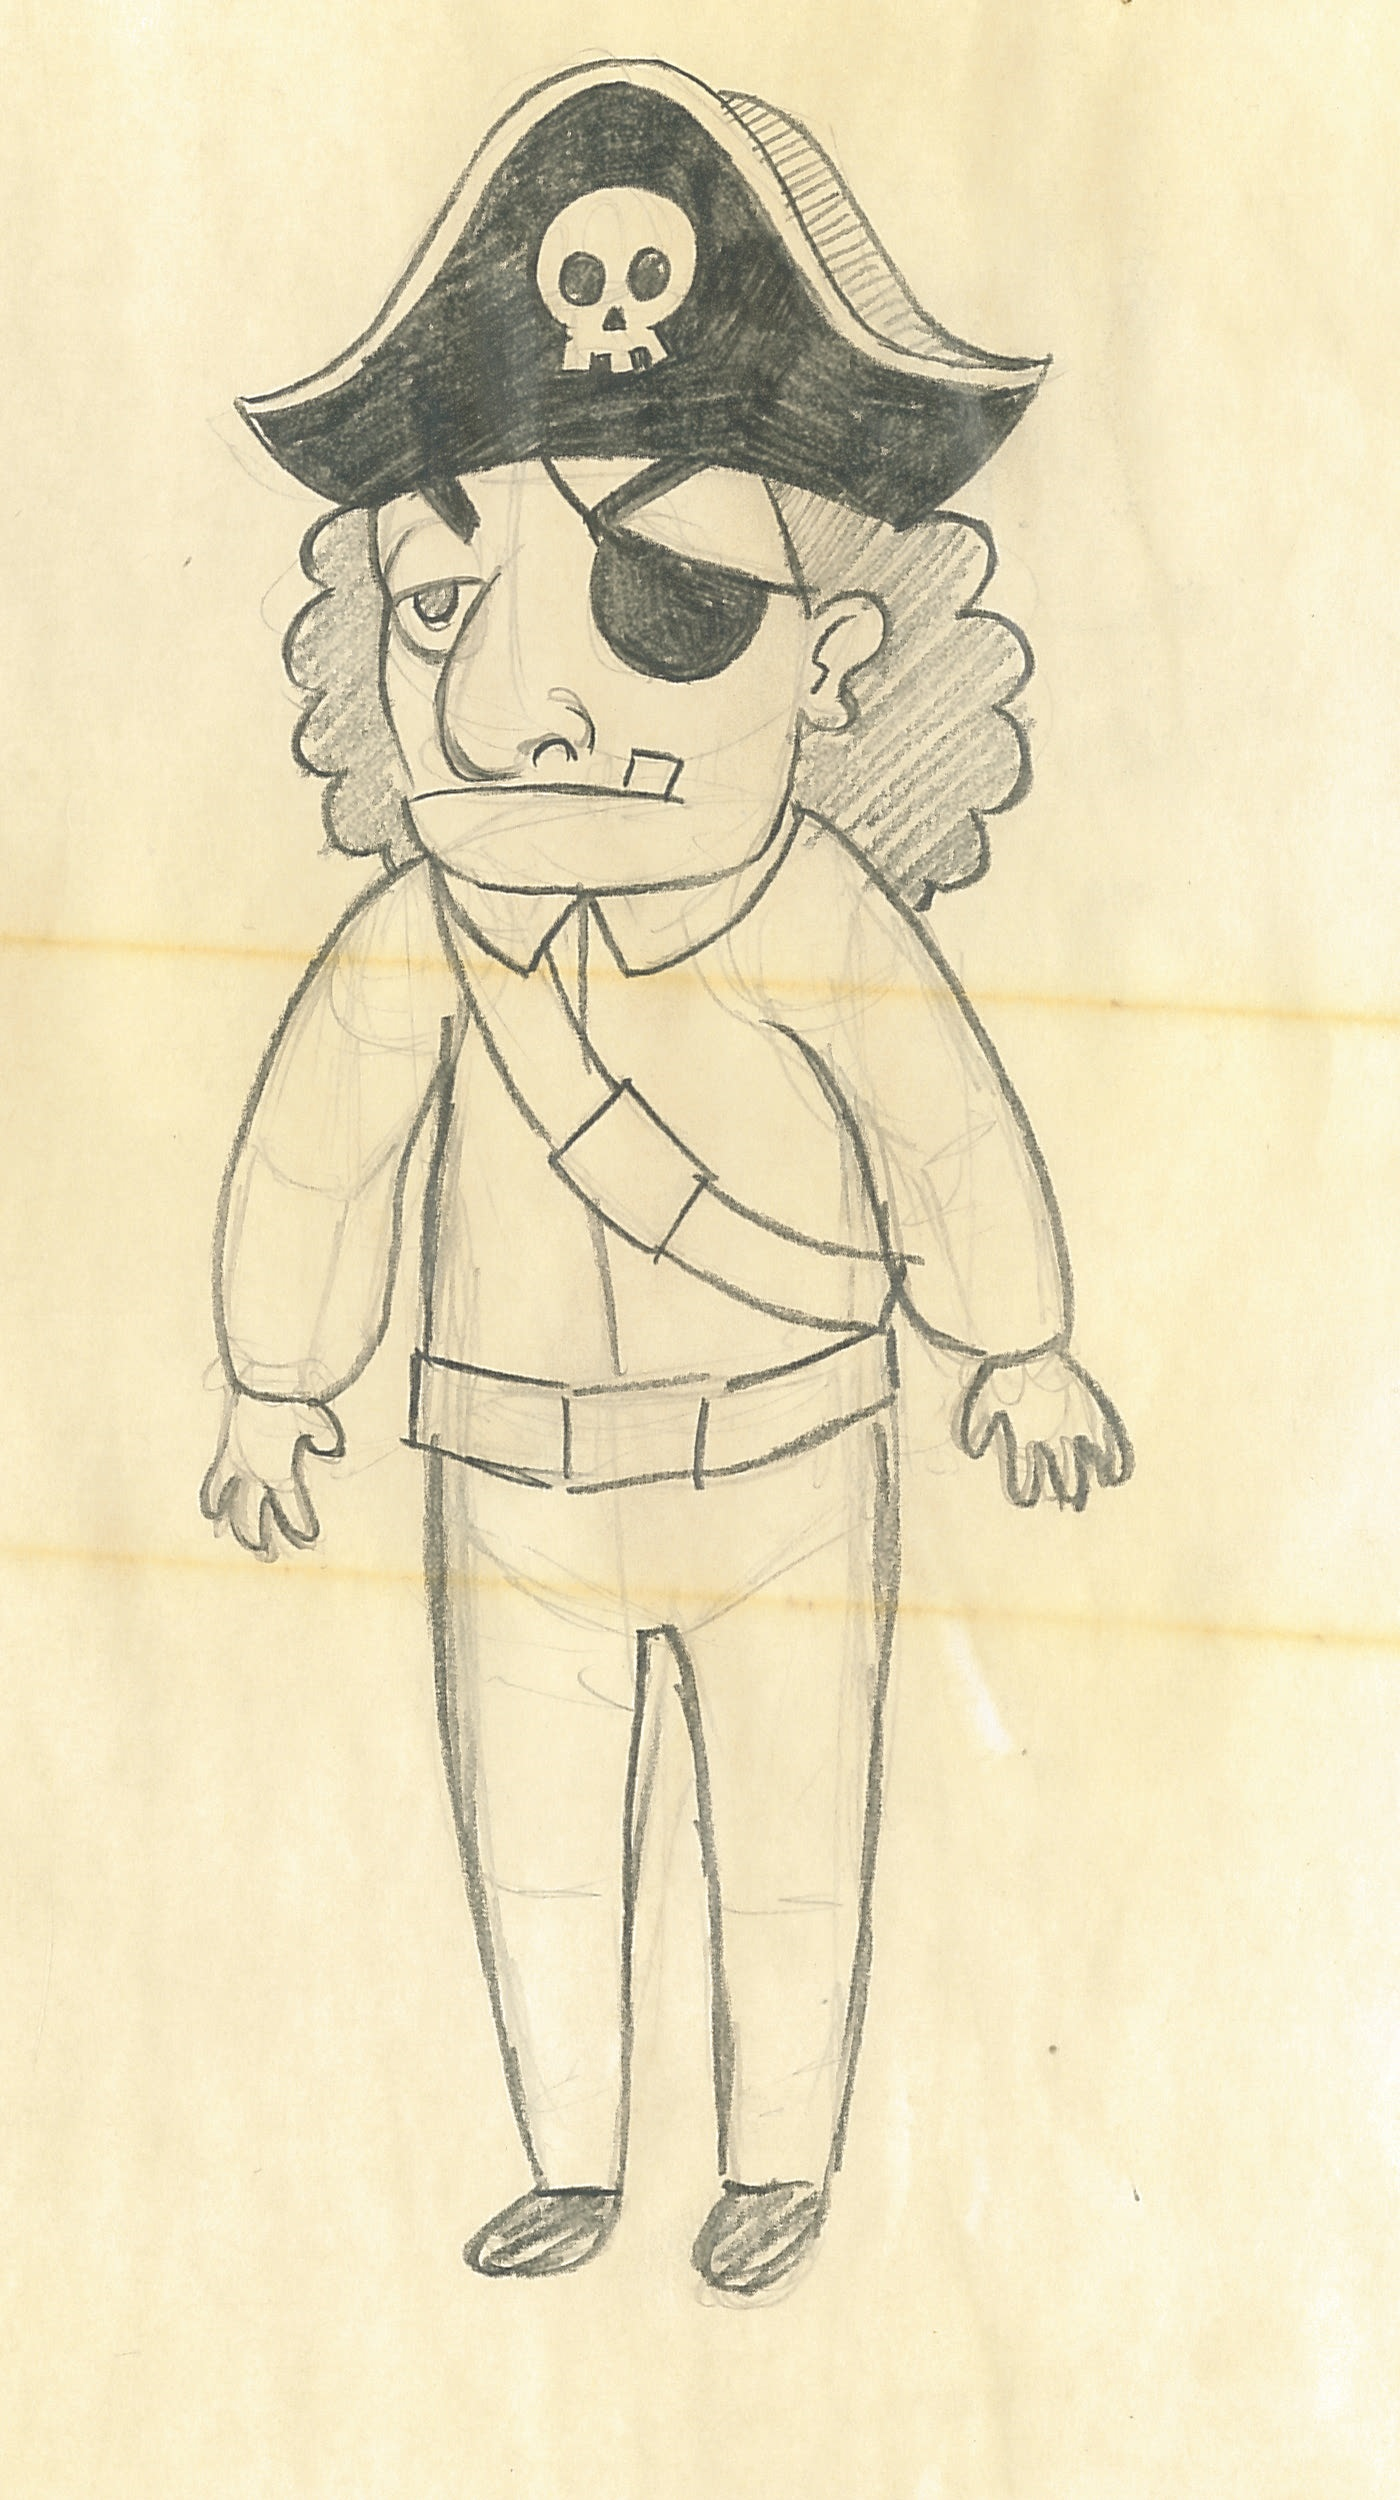
\includegraphics[width=\textwidth]{figures/pirate_concept_3.png}\caption{ \label{fig:pirate_concept_3}}
    \end{subfigure}
    \caption{Concept art of the pirate characters}\label{fig:pirate_concepts}
\end{figure}

In the end, the concept pictured in Figure \ref{fig:pirate_concept_2} was decided upon, in part due to its large torso; if the shirt and bandana are a certain colour, that colour would take up a relatively large percentage of the character's surface, allowing for it to be easily seen by the players, even with several characters present on the screen. This is true for any character on screen, since an isometric perspective is used. This means that any playable character on screen will not become smaller when placed further away, and all characters will take up the same amount of screen no matter the position.

\section{3D graphics}

\subsection{Modeling}
The models for this game are built and animated using Autodesk Maya \cite{Autodesk}, and consist of transformed primitives, such as spheres and cylinders. For example, the head of the player-controlled pirate character is a transformed sphere, and the torso as well as the limbs consist of cylinders. The trunks of the palm trees are created from cylinders, and their leaves from planes. All four pirate characters have identical meshes, seen in Figure \ref{fig:pirate_mesh}.

\begin{figure}[h!]
	\centering
	\includegraphics[width=0.9\textwidth]{figures/pirate_mesh.png}
	\caption{Pirate mesh: front, side and back view \label{fig:pirate_mesh}}
\end{figure}

The components of the pirate mesh were transformed based on two reference images of the character design, assigned to two image planes, one showing a frontal view of the character, and one showing a side view. These planes can be seen in Figure \ref{fig:pirate_planes}. However, small changes were made during modeling, such as the short pigtails, which were changed into longer braids in the final version.

\begin{figure}[h!]
	\centering
	\includegraphics[width=0.7\textwidth]{figures/pirate_planes.png}
	\caption{Pirate mesh: front, side and back view \label{fig:pirate_planes}}
\end{figure}

The interactive objects were not created using this technique, but rather modelled "free-hand". The lack of planes to built from is seen in Figure \ref{fig:palmtree_mesh}. Like the character, the design of these objects aim for simplicity, rather than realism.

\begin{figure}[h!]
	\centering
	\includegraphics[width=0.7\textwidth]{figures/palmtree_mesh.png}
	\caption{Palm tree mesh \label{fig:palmtree_mesh}}
\end{figure}

\subsection{Textures}
Each pirate is assigned a \textit{lambert} material with a simple texture applied to it. This type of material uses a model for diffuse reflection. This means that light reflects off this material in all directions, which makes the material look matte. This is useful as the textures are made to look like cartoonish skin and clothes, which means that reflective highlighting is something to avoid. The textures are very similar (simple face, light skin, neutrally coloured shorts), but they differ in the colour of each pirate's bandana and shirt. The colours of the four characters are red, green, yellow, and blue, as pictured in Figure \ref{fig:pirate_rainbow}. The green colour specifically is chosen, so that it is not too similar to the yellow colour --- the two were reviewed internally by a colour deficient person, who often has trouble discerning between light green and yellow colours. This person was able to easily discern between the yellow and green pirates.

\begin{figure}[h!]
	\centering
	\includegraphics[width=\textwidth]{figures/pirate_rainbow.png}
	\caption{All four player colours \label{fig:pirate_rainbow}}
\end{figure}

The texture was applied to the pirates using UV mapping; the geometry is flattened onto a two-dimensional coordinate system. Based on this flattened-out UV-map, an image containing all the necessary colours was created. An example of such a UV map (specifically for the red pirate) is seen in Figure \ref{fig:uv_map}.

\begin{figure}[h!]
	\centering
	\includegraphics[width=\textwidth]{figures/uv_map.png}
	\caption{The UV map for a pirate \label{fig:uv_map}}
\end{figure}

The interactive objects have likewise been textured. These objects can be seen in Figure \ref{fig:objects}.

\begin{figure}[h!]
    \centering
    \begin{subfigure}[b]{0.3\textwidth}
    	\centering
        \includegraphics[scale=0.2]{figures/fern.png}\caption{A fern\label{fig:fern}}
    \end{subfigure}
    \begin{subfigure}[b]{0.3\textwidth}
    	\centering
        \includegraphics[scale=0.2]{figures/skull.png}\caption{A skull\label{fig:skull}}
    \end{subfigure}
    \begin{subfigure}[b]{0.3\textwidth}
    	\centering
        \includegraphics[scale=0.2]{figures/PalmTree.png}\caption{A palm tree\label{fig:palmtree}}
    \end{subfigure}
\caption{The interactive objects}\label{fig:objects}
\end{figure}

\pagebreak
\section{Rigging and animation}
In order to animate the models, they have all been rigged. A skeleton is created and assigned to a model, with joints at the places where the model in question should be able to bend. For example, the pirate model seen in Figure \ref{fig:rigged_pirate} has a skeleton assigned to it, with joints at its shoulders, wrists, knees, et cetera. This is called 'binding the skin' to the skeleton. The joints are arranged in a hierarchy, shown in Figure \ref{fig:hierarchy}. The hierarchy is arranged such that if the shoulder bends, the rest of the arm will follow, et cetera. When skinning, we had to define the skin's \textit{max influence}, which determines how many skeleton joints and objects that can influence any given point on the model. The default value in Maya for this setting is 5, but we lowered it to 3. This is because the models are made to be imported into the game engine Unity \cite{unity} and it does not support skins with max influences higher than 3.

\begin{wrapfigure}{r}{0.5\textwidth}
  \begin{center}
    \includegraphics[scale=1]{figures/hierarchy.png}
  \end{center}
  \caption{The joint hierarchy}\label{fig:hierarchy}
\end{wrapfigure}

Once the skeleton is built, each joint's \textit{weight} is painted onto the model. The weight of a joint controls which parts of the body move as the joint is rotated, and how much. Figure \ref{fig:elbow_pirate} shows weights painted in the pirate's left elbow. Furthermore, limits are set for each joint so that they do not bend too far, or bend in the wrong direction. For example, the pirate's knees can only bend on the y-axis, and only towards the rear.

\begin{figure}[h!]
	\centering
	\begin{subfigure}[b]{0.45\textwidth}
		\centering
		\includegraphics[scale=0.6]{figures/rigged_pirate.png}
		\caption{The rigged skeleton}
		\label{fig:rigged_pirate}
	\end{subfigure}
	\begin{subfigure}[b]{0.45\textwidth}
		\centering
		\includegraphics[scale=0.6]{figures/elbow_pirate.png}
		\caption{The pirate's elbow, with weights}
		\label{fig:elbow_pirate}
	\end{subfigure}
	\caption{A rigged version of the pirate model}
	\label{fig:riggin}
\end{figure}

With the skeleton properly set up, the model can be posed in different positions, allowing for animation using key frames. Key frames mark the start and end points of a smooth transition between two poses. For this project, the models are posed in Autodesk Maya, which automatically generates a smooth transition once the key frames have been set. When setting the key frames, the model is posed using the rigged joints. This method is referred to as \textit{forward kinematics}, where the animator controls each specific joint. This stands in contract to \textit{inverse kinematics}, where the animator sets the position of an element --- a hand, for example --- and calculations are done by the computer to determine the position of the remainder of the arm.

The pirate model has three animations with 4-6 key frames, all of which can be seen in Figure \ref{fig:key_frames}. Likewise, the interactive objects each have an animation that will play when they are searched.

\begin{figure}[h!]
	\centering
	\begin{subfigure}[b]{\textwidth}
		\centering
		\includegraphics[scale=0.25]{figures/walk_cycle.png}
		\caption{Walk cycle}
		\label{fig:walk_cycle}
	\end{subfigure}
	
	\begin{subfigure}[b]{\textwidth}
		\centering
		\includegraphics[scale=0.25]{figures/attack_anim.png}
		\caption{Attack animation}
		\label{fig:attack_anim}
	\end{subfigure}
	
	\begin{subfigure}[b]{\textwidth}
		\centering
		\includegraphics[scale=0.25]{figures/search_anim.png}
		\caption{Search animation}
		\label{fig:search_anim}
	\end{subfigure}
	\caption{Key frames for the animations of the pirate}
	\label{fig:key_frames}
\end{figure}

\section{Interface elements}
For the purposes of testing, several images for visual feedback have been created for different types of feedback on two screens. The images signalling that it is now a certain player's turn consist mainly of that player's colour, as seen in Figure \ref{fig:yellow_turn}, in which the yellow player's signal is shown. The intent is that the player's attention is quickly drawn to the image and that it is quickly communicated that it is a given player's turn.

\begin{figure}[h!]
	\centering
	\includegraphics[width=0.7\textwidth]{figures/yellowturn.png}
	\caption{Visual feedback for yellow player's turn}
	\label{fig:yellow_turn}
\end{figure}

When a fight is about to commence, the image seen in Figure \ref{fig:get_ready} shows up. It is black with highly contrasting colours in order to quickly catch the players' visual attention without being biased in any player's direction.

\begin{figure}[h!]
	\centering
	\includegraphics[width=0.7\textwidth]{figures/getready.png}
	\caption{Visual feedback warning players that a fight will commence}
	\label{fig:get_ready}
\end{figure}

The actual fighting screen, which appears during a fight sequence between two players, is unsaturated. Ideally by this point, the player's attention is already aimed at the phone screen, either nudged by the tactile feedback or the "Get ready to FIGHT!" image depending on the test. The three combat buttons are of a bright orange colour to make them stand out from the background image and therefore immediately grasp the player's attention towards them. The fighting screen can be seen in Figure \ref{fig:fight}. The player needs to press the buttons in the correct order and faster than the opponent to win the combat. 

\begin{figure}[h!]
	\centering
	\includegraphics[width=0.7\textwidth]{figures/fight.png}
	\caption{The fight screen}
	\label{fig:fight}
\end{figure}

\begin{figure}[h!]
	\centering
	\includegraphics[width=0.7\textwidth]{figures/WonPhone}
	\caption{Winning screen for yellow player}
	\label{fig:winning}
\end{figure}

\begin{figure}[h!]
	\centering
	\includegraphics[width=0.7\textwidth]{figures/LostPhone}
	\caption{Losing screen for green player}
	\label{fig:losing}
\end{figure}

After the combat results are clear, the fight screen changes to either a winning or a loosing screen depending on the outcome. The winning screen can be seen in Figure\ref{fig:winning}, and the loosing screen can be seen in Figure\ref{fig:losing}.

\section{Phone interface}
The smart phone has three primary screens besides the fight screen: the planning screen, the waiting screen and the map screen. Only two out of the three were complete at the end of this project, the planning as seen on Figure \ref{fig:plan}, and the waiting screen a seen on Figure \ref{fig:wait}. 

\begin{figure}[h!]
	\centering
	\includegraphics[width=0.7\textwidth]{figures/planningScreen.png}
	\caption{The planning screen}
	\label{fig:plan}
\end{figure}


\begin{figure}[h!]
	\centering
	\includegraphics[width=0.7\textwidth]{figures/waitingScreen.png}
	\caption{The waiting screen}
	\label{fig:wait}
\end{figure}

All the phone screens except for the combat screen share the same background. The background was chosen to resemble old paper, like a traditional treasure map. This determined the rest of the colour scheme, with the buttons being either white or differing shades of beige. The colour scheme was also chosen to not be too eye-catchy in order not to direct attention to any particular thing, with the exception of the ready button that is much brighter than everything else in order to catch attention. All screens  have the AirConsole logo in the middle of the top of the screen during gameplay. 

There are ten objects on the screen, eight of which are interactable.
Going left to right, from top to bottom, the first object is the button which will open the map screen. It is a half circle with a simple illustration of a treasure map inside to indicate that the map screen will appear if this button is pressed. It is not interactable since the map screen is not implemented for this version of the game. Underneath that button are two numbers representing the number of map pieces: the left one shows the players current amount of map pieces and the right shows the total map pieces necessary to win.

The next objects are the two boxes in the top of the screen which are the planning boxes. They represent the first and second actions the player can execute. They are automatically chosen in the order 1-2, but it is possible to plan otherwise by first clicking on the number and then clicking on the desired action. When clicking an action, the icon will show up in the chosen planning box. The planning boxes have a transparent background to indicate that they are not buttons. 

Right next to them, there is another box of the same shape with a transparent backgroud, that contains the timer. It indicates how much time, in seconds, the player has left to complete the turn. Besides that, a phrase "TIME LEFT" is also put there in order to avoid the player's confusion.

Onwards, there are the movement buttons placed in a two by two grid. Since the arena is in an isometric angle and is seen from the corner, the movement arrows are diagonal, not horizontal and vertical. They have a light beige colour called \textit{cornsilk} in CSS. 

The next object is the interact button. It is illustrated with a magnifying glass, since the interact action is used for searching an object for map pieces. Its background colour is different from that of the the movement buttons to distinguish it from them and make it clear that it is a different action. The colour is called \textit{moccasin} in CSS, and was also chosen for not being too eye-catching, but still different enough from the others. 

Finally there is the ready button. This is a green check mark on a pure white background, which makes it the object that stands out the most on the screen. It is also the biggest object on the screen illustrating its importance. A turn will not execute if this button is not pressed. 

The waiting screen has all the same objects as the planning screen, except for the timer. On top of it all is a transparent background with the word "WAITING" taking up most of the screen. This makes the buttons non-interactable, with the exception for the map button, which, if it had been implemented, would be interactive. The font for the "WAITING" and all the other text is in a font called \textit{PiratesBay}, which is free to use. This was used to give a piratelike feel to the controller.